% Summary charts for report.tex. Run scripts/generate_report_figures.py to refresh.
\begin{figure}[htbp]
\centering
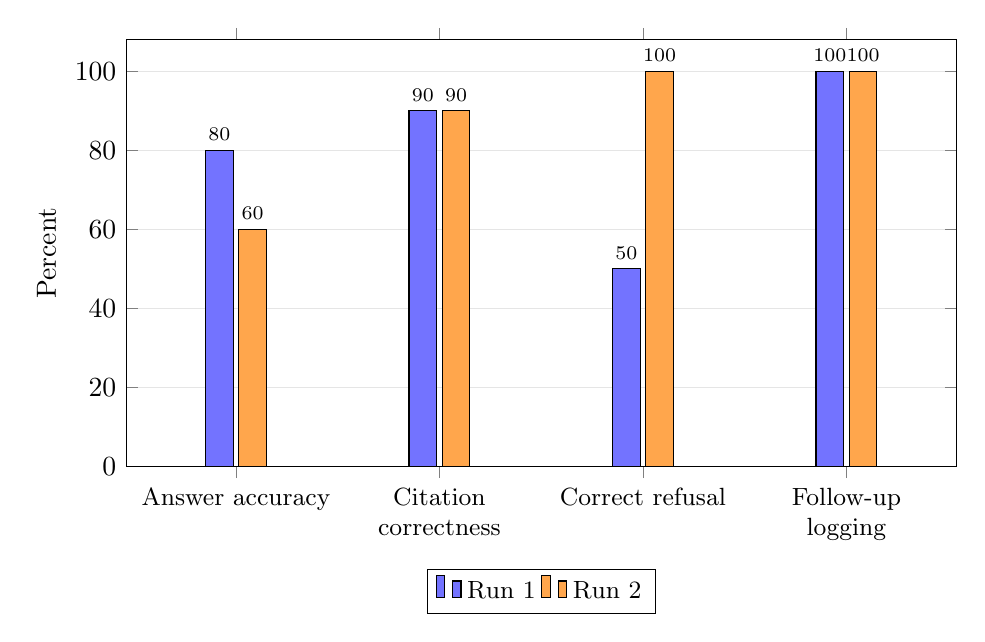
\begin{tikzpicture}
\begin{axis}[
  ybar, bar width=10pt, width=\textwidth, height=7cm,
  ymin=0, ymax=108, ylabel={Percent},
  symbolic x coords={accuracy,citation,refusal,logging}, xtick=data,
  xticklabels={Answer accuracy,Citation correctness,Correct refusal,Follow-up logging},
  x tick label style={text width=2.4cm,align=center,font=\small},
  ymajorgrids=true, grid style={gray!20},
  nodes near coords, nodes near coords style={font=\scriptsize},
  enlarge x limits=0.18,
  legend style={at={(0.5,-0.24)},anchor=north,legend columns=2,font=\small},
]
\addplot[fill=blue!55] coordinates {(accuracy,80) (citation,90) (refusal,50) (logging,100)};
\addlegendentry{Run 1}
\addplot[fill=orange!70] coordinates {(accuracy,60) (citation,90) (refusal,100) (logging,100)};
\addlegendentry{Run 2}
\end{axis}
\end{tikzpicture}
\caption{Qwen3 on the main 28-prompt set. Accuracy and citation correctness use 20 in-scope prompts per run; refusal and logging use eight out-of-scope prompts. Refusal bars use the entered CSV grades.}
\label{fig:qwen-main}
\end{figure}

\begin{figure}[htbp]
\centering
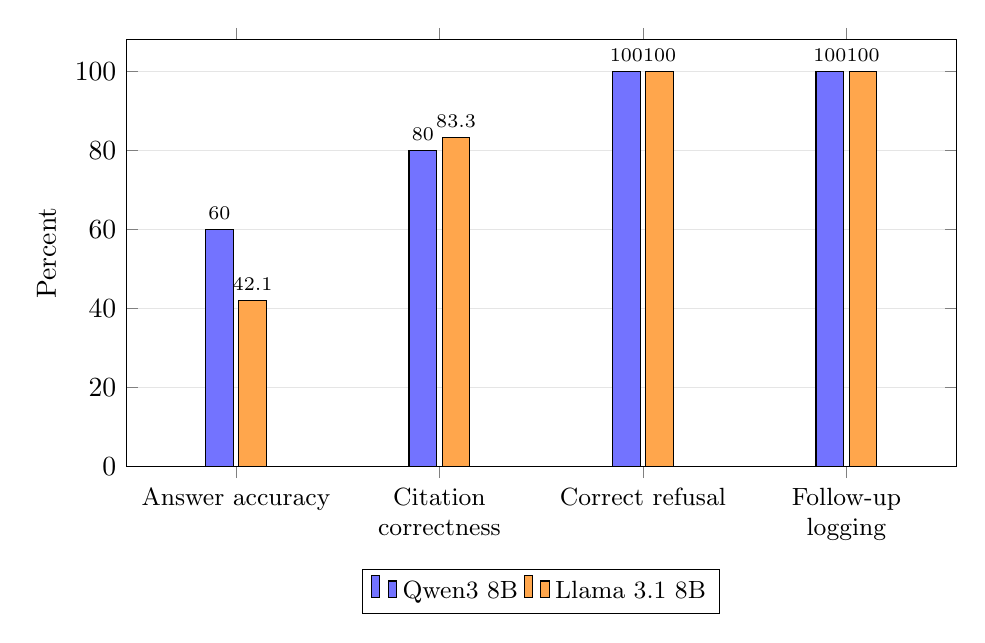
\begin{tikzpicture}
\begin{axis}[
  ybar, bar width=10pt, width=\textwidth, height=7cm,
  ymin=0, ymax=108, ylabel={Percent},
  symbolic x coords={accuracy,citation,refusal,logging}, xtick=data,
  xticklabels={Answer accuracy,Citation correctness,Correct refusal,Follow-up logging},
  x tick label style={text width=2.4cm,align=center,font=\small},
  ymajorgrids=true, grid style={gray!20},
  nodes near coords, nodes near coords style={font=\scriptsize},
  enlarge x limits=0.18,
  legend style={at={(0.5,-0.24)},anchor=north,legend columns=2,font=\small},
]
\addplot[fill=blue!55] coordinates {(accuracy,60) (citation,80) (refusal,100) (logging,100)};
\addlegendentry{Qwen3 8B}
\addplot[fill=orange!70] coordinates {(accuracy,42.1) (citation,83.3) (refusal,100) (logging,100)};
\addlegendentry{Llama 3.1 8B}
\end{axis}
\end{tikzpicture}
\caption{Pooled results on the matched 14-prompt LLM subset, two runs per model. Percentages use nonblank grades; the Llama answer and citation rates therefore have smaller denominators.}
\label{fig:llm-subset}
\end{figure}

\begin{figure}[htbp]
\centering
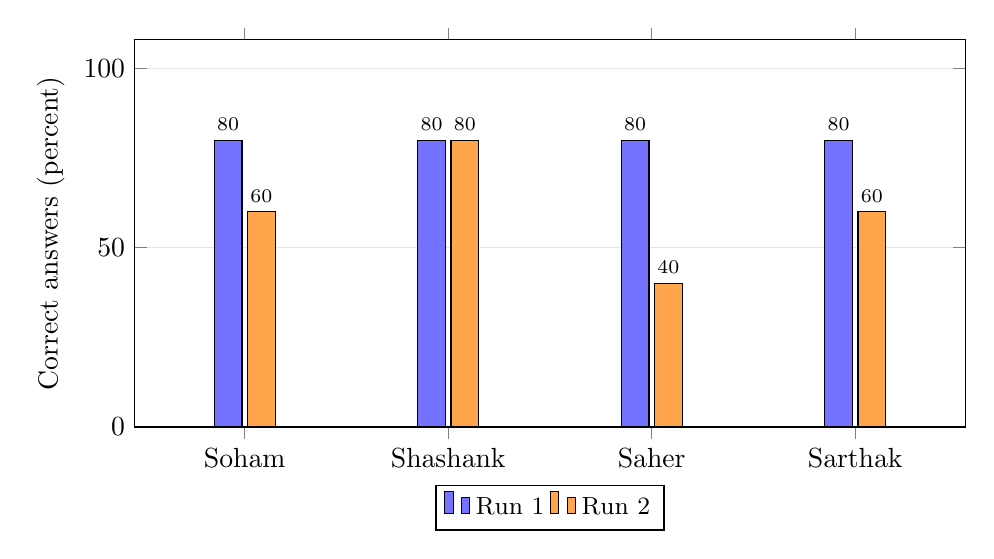
\begin{tikzpicture}
\begin{axis}[
  ybar, bar width=10pt, width=\textwidth, height=6.5cm,
  ymin=0, ymax=108, ylabel={Correct answers (percent)},
  symbolic x coords={soham,shashank,saher,sarthak}, xtick=data,
  xticklabels={Soham,Shashank,Saher,Sarthak},
  ymajorgrids=true, grid style={gray!20},
  nodes near coords, nodes near coords style={font=\scriptsize},
  enlarge x limits=0.18,
  legend style={at={(0.5,-0.15)},anchor=north,legend columns=2,font=\small},
]
\addplot[fill=blue!55] coordinates {(soham,80) (shashank,80) (saher,80) (sarthak,80)};
\addlegendentry{Run 1}
\addplot[fill=orange!70] coordinates {(soham,60) (shashank,80) (saher,40) (sarthak,60)};
\addlegendentry{Run 2}
\end{axis}
\end{tikzpicture}
\caption{Correct-answer rate by participant group on the main Qwen3 prompt set. Each group has five in-scope questions.}
\label{fig:group-accuracy}
\end{figure}
